\documentclass[11pt,a4paper]{article}

\usepackage[utf8]{inputenc}
\usepackage[T1]{fontenc}
\usepackage[margin=2.3cm]{geometry}
\usepackage{lmodern}
\usepackage{microtype}
\usepackage{booktabs}
\usepackage{graphicx}
\usepackage{float}
\usepackage{caption}
\usepackage{xcolor}
\usepackage{hyperref}
\usepackage{enumitem}
\usepackage{titlesec}
\usepackage{fancyhdr}

\definecolor{ink}{HTML}{0B0B0B}
\definecolor{quiet}{HTML}{52514E}
\hypersetup{colorlinks=true, linkcolor=ink, urlcolor=blue!50!black, citecolor=ink}

\titleformat{\section}{\Large\bfseries\color{ink}}{\thesection}{0.8em}{}
\titleformat{\subsection}{\large\bfseries\color{ink}}{\thesubsection}{0.6em}{}
\titlespacing*{\section}{0pt}{1.6em}{0.6em}
\titlespacing*{\subsection}{0pt}{1.1em}{0.4em}

\pagestyle{fancy}
\fancyhf{}
\renewcommand{\headrulewidth}{0pt}
\fancyfoot[C]{\small\color{quiet}\thepage}

\captionsetup{font=small,labelfont=bf,textfont={color=quiet}}
\setlength{\parskip}{0.5em}
\setlength{\parindent}{0pt}

\newcommand{\pct}[1]{#1\,\%}

\title{\bfseries Bid-Rigging Detection Benchmark:\\Project Report}
\author{}
\date{As of 28 October 2026}

\begin{document}
\maketitle
\thispagestyle{empty}

% ---------------------------------------------------------------- PREFACE
\section*{Preface}

This project asks one question: which bid-rigging schemes can a regulator detect from public bid data alone, including schemes the detector has never seen? It builds a benchmark of simulated procurement markets with eight imposed cartel schemes, a detector, and a locked evaluation protocol. It then checks the detector on real cartel cases from three countries.

\textbf{What the project does.} It simulates repeated first-price procurement tenders in which the same firms meet again and again. A cartel scheme (rotation, cover bidding, price fixing and five others) is imposed on some markets; the rest are honest. The detector reads only what a buyer can see: each bid, who placed it, and the buyer's published cost estimate. It then gives each market a suspicion score. Its core idea is to look at \emph{who moves with whom}: whether particular firms' bids rise and fall together, track each other closely, or avoid each other more than chance would allow in that market.

\textbf{Why it pivoted from the earlier project.} The earlier project trained 20 reinforcement-learning firms (one shared PPO policy) to bid while a Bayesian sequential regulator watched the bids and fined suspects. The aim was to see whether firms learn to collude and whether the regulator catches them. Cartels formed briefly and collapsed to about 0--2 members within roughly ten training iterations. Measured payoffs explained why: against any competitive fringe, cartel members earned less than honest firms even with no fines, and only a cartel of all 20 firms gained, by about +0.5 per round. Changing frictions, pricing rules, the strategy menu and the number of firms did not change this. With almost no cartels to find, the detection question could not be answered.

The pivot separates the two questions. Whether agents learn to collude was answered (in that environment, no). Whether collusion can be detected matters regardless, because real authorities face cartels that already exist. The new project therefore imposes cartels directly, as forensic studies do, and puts the effort into a rigorous detection test.

\begin{table}[H]
\centering
\small
\begin{tabular}{@{}p{2.6cm}p{5.6cm}p{5.6cm}@{}}
\toprule
& Earlier project & This project \\
\midrule
Firms & 20 learning agents (PPO) choosing strategies each round & Rule-based honest firms; cartels imposed by scheme \\
Collusion & Had to emerge; it did not persist & Eight schemes plus a negative control, randomised per market \\
Detector & Bayesian sequential regulator on price-level screens & Identity-based dependence features, screens and a sequential layer, combined by gradient boosting \\
Test & Mostly in-distribution & Each scheme held out; unseen market sizes and spreads; locked test run once \\
Main finding & Collusion did not pay, so cartels collapsed & Four schemes detected reliably; four are not \\
\bottomrule
\end{tabular}
\caption{The earlier and current projects compared.}
\end{table}

Lessons from the earlier project shaped the new design. A price-level screen had flagged honest firms with high markups, so the new features cancel the price level. A calibration mismatch had caused 70\,\% false alarms, so thresholds are now set on data from the same generator as the test. An earlier AUC bug led to every metric being tested on separated, reversed and tied data before use.

% ---------------------------------------------------------------- METHOD
\section{How the study was run}

\textbf{Simulated markets.} Each market has 6--30 firms that meet in 20--60 sealed-bid tenders; the lowest bid wins. Every firm has a persistent cost efficiency, strengths for certain tender types, and a capacity backlog that raises its cost after recent wins. The backlog gives honest markets rotation-like patterns on purpose, so the detector cannot win by flagging any rotation. The buyer publishes a noisy cost estimate per tender, built from project size only, never from firms' costs. Honest firms bid cost times a market-wide markup of 0--25\,\%, plus a small firm-specific markup and competition shading.

\textbf{Eight cartel schemes}, each with randomised parameters and imposed on a share of firms (the rest stay honest):
\begin{enumerate}[leftmargin=2em]
\item Rotation: members take turns as the designated winner.
\item Cover bidding: the cheapest member wins; the others bid just above it.
\item Complementary bidding: losing members bid fixed multiples of the estimate.
\item Price fixing: members bid an agreed price, at low, mid or high levels.
\item Partial cartel with a fringe: only 2--3 firms collude among many honest ones.
\item Noisy or defecting cartel: cover bidding with noise; members sometimes undercut.
\item Intermittent cartel: active only in one window of 30--60\,\% of the tenders.
\item Bid suppression: members withdraw so the designated winner faces fewer bids.
\end{enumerate}

A ninth scheme, uniform-markup collusion (every firm raises prices by 30--60\,\%), is kept as a negative control. Without cost data it looks the same as honest firms with higher costs, so no bid-only detector should catch it.

\textbf{The detector.} It turns a market's bids into four groups of features, then a gradient-boosted classifier combines them into one suspicion score:
\begin{itemize}
\item \emph{Literature screens:} coefficient of variation, skewness, kurtosis, relative distance, bid gaps and spread, per tender, averaged over the market.
\item \emph{Dependence features (the core).} Each bid is expressed relative to the estimate and the tender's median bid, which removes price level and markups. The features then measure pair co-movement, cover-bid tracking, wins that are inconsistent with a firm's cost strength, and firms that avoid bidding together. Each is compared with the same market shuffled two ways (bids swapped between firms within a tender; each firm's bids reordered across tenders), so it asks whether the pattern is stronger than chance in this market.
\item \emph{Change scans:} whether behaviour shifts at some point in the market's history.
\item \emph{A sequential layer:} a two-state Bayesian filter and a CUSUM over the tenders.
\end{itemize}

\textbf{The test protocol}, fixed before any results were seen:
\begin{itemize}
\item Leave one scheme out: each scheme is scored by a model trained without it, so every result is for a cartel type the detector never saw.
\item Market shifts: test markets have unseen sizes (6--7 and 25--30 firms) and unseen cost spreads, plus honest stress sets (markups of 20--25\,\%, strong capacity effects, noisy estimates).
\item Three splits: tuning to fit models, validation to choose designs, and a locked test run once. The script refuses to run the same frozen design twice.
\item 10 random seeds, and 95\,\% bootstrap confidence intervals on every headline number.
\item The alarm threshold is set at 5\,\% false alarms on separate honest calibration markets from the same generator.
\end{itemize}

\textbf{Reading the numbers.}
\begin{itemize}
\item \emph{AUC:} the probability that the detector ranks a randomly chosen cartel market above a randomly chosen honest one. 0.5 is a coin flip, 1.0 is perfect separation, and below 0.5 means honest markets look more suspicious than cartels. It does not depend on the alarm threshold.
\item \emph{False-alarm rate:} the share of honest markets flagged at the chosen threshold.
\item \emph{Precision@10\,\%:} of the 10\,\% of markets ranked most suspicious, the share that are truly cartels. This mirrors an authority that investigates the top of a list.
\item \emph{Detector AUC} means the proposed model's AUC; screens-only AUC is the same kind of model using only the literature screens.
\end{itemize}

% ---------------------------------------------------------------- RESULTS
\section{Results at a glance}

Three of the four criteria, fixed before the test was run, are met on the locked test. The strictest one, that every unseen scheme reaches AUC 0.85, is not. The locked run used the frozen design \texttt{full\_gbm}, 10 seeds and 1{,}000 bootstrap resamples. Confidence intervals are in brackets.

\begin{table}[H]
\centering
\small
\begin{tabular}{@{}p{5.2cm}p{7.6cm}p{1.6cm}@{}}
\toprule
Criterion (fixed in advance) & Locked-test result & Met \\
\midrule
Every held-out scheme reaches AUC $\ge$ 0.85, including unseen sizes and spreads & 4 of 8 pass (worst condition $\ge$ 0.92); partial cartel 0.672, bid suppression 0.744, noisy cartel 0.823, intermittent 0.849 at unseen spreads & No \\
False alarms $\le$ 10\,\% on every honest test set & Highest 0.075 [0.050, 0.105], on unseen market sizes & Yes \\
Beats the literature baselines, with the confidence interval excluding them & AUC 0.870 vs 0.803 for the screens model; difference +0.067 [0.060, 0.074] & Yes \\
Precision@10\,\% above the base rate, interval excluding it & Lowest 0.378 [0.335, 0.418] against a base rate of 0.167 & Yes \\
\bottomrule
\end{tabular}
\caption{Pre-registered criteria and their locked-test outcome.}
\end{table}

Because one criterion failed, the result is presented as a benchmark with an honest partial negative finding rather than a solved detection problem. The negative control behaved as theory predicts: uniform-markup collusion scored AUC 0.478 [0.450, 0.503], and only 4.7\,\% of those markets were flagged.

\subsection{Results by cartel scheme}

Rotation, price fixing, complementary bidding and cover bidding are detected reliably even though the model never saw them. The four quieter schemes are not.

\begin{figure}[H]
\centering
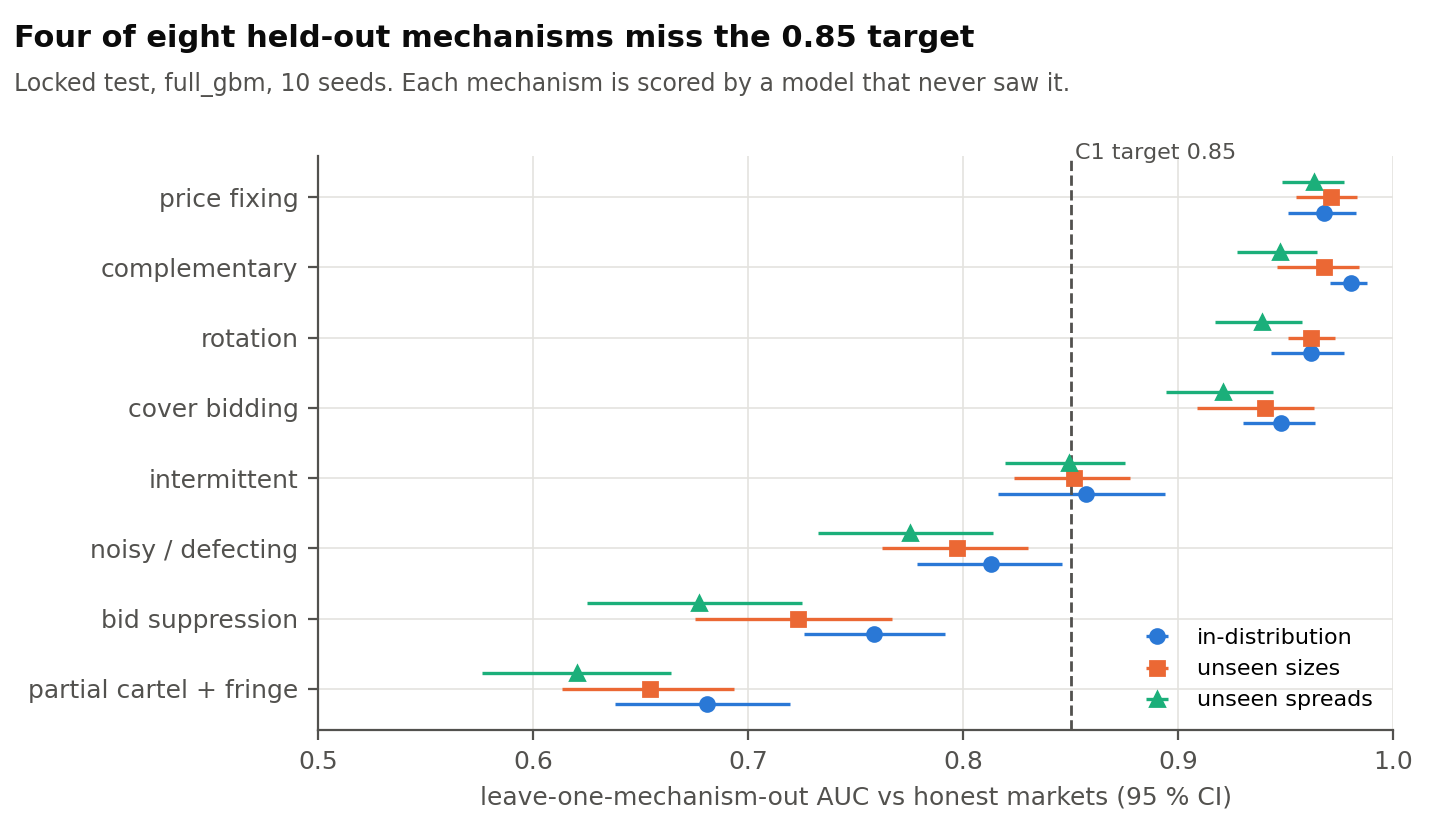
\includegraphics[width=\linewidth]{../figures/fig1_locked_auc_by_mechanism.png}
\caption{Held-out AUC per scheme and market condition (locked test, 95\,\% CIs). The dashed line is the 0.85 target.}
\end{figure}

Each row is one scheme, scored by a model trained on the other seven. The three dots per row are the three market conditions: sizes and cost spreads seen in training, unseen market sizes, and unseen cost spreads. Unseen spreads are the hardest condition for every scheme, so the detector loses some accuracy when cost dispersion moves outside its training range.

The detected schemes all leave a strong trace between specific firms: covers that track the winner, bids at a common level, or wins that rotate against cost strength. The missed ones leave weak or diluted traces. A 2--3 firm cartel in a large market sits in one or two firm pairs. Noisy and defecting cartels blur the cover pattern. Bid suppression shows mainly as missing bids, which the model cannot learn when that scheme is held out. The intermittent cartel misses the target by 0.001, at unseen spreads only.

Ranking still works for every scheme. Among the 10\,\% of markets ranked most suspicious, the share that are truly cartels ranges from 0.378 (partial cartel) to 0.983 (price fixing), against a base rate of 0.167.

\subsection{Against the standard collusion screens}

\begin{figure}[H]
\centering
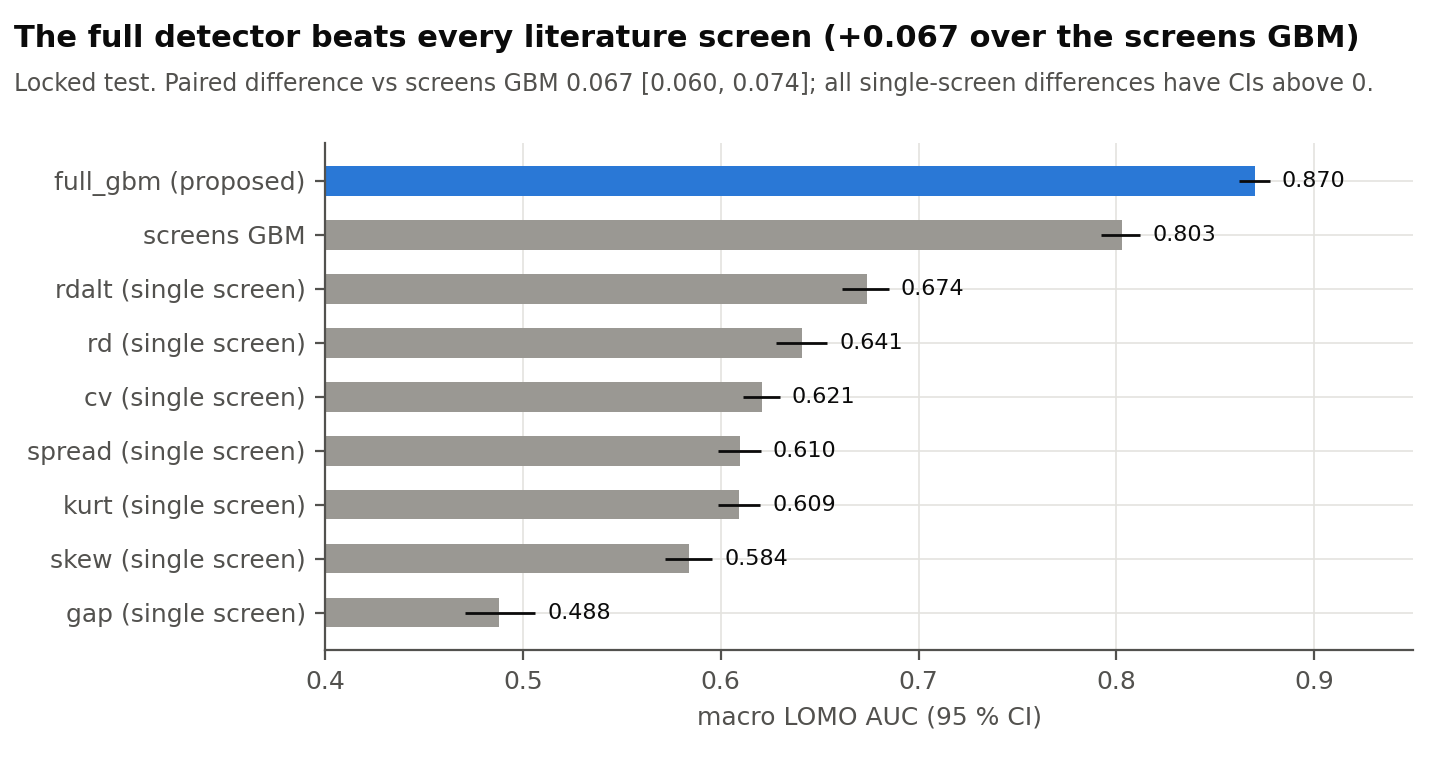
\includegraphics[width=0.9\linewidth]{../figures/fig2_locked_vs_baselines.png}
\caption{Macro AUC over the eight held-out schemes, with 95\,\% CIs.}
\end{figure}

The proposed detector beats the strongest literature baseline by 0.067 AUC, and the confidence interval of that gain, [0.060, 0.074], is well above zero. Macro AUC is the average over the eight held-out schemes, each scored by a model that never saw it. The screens model is the fair comparison: the same gradient-boosting classifier, given only the seven literature screens. Its gap to the proposed detector is the value of the dependence features. Every single screen is also beaten, by 0.196 (RD-alt) to 0.382 (gap); every difference was paired on the same markets, and each confidence interval excludes zero.

Single screens do poorly here because they measure the spread and shape of one tender's bids. Those depend on cost dispersion and market size, which change between training and test markets. The dependence features compare each market with its own shuffled versions, so they hold up better under those shifts.

\subsection{False alarms}

\begin{figure}[H]
\centering
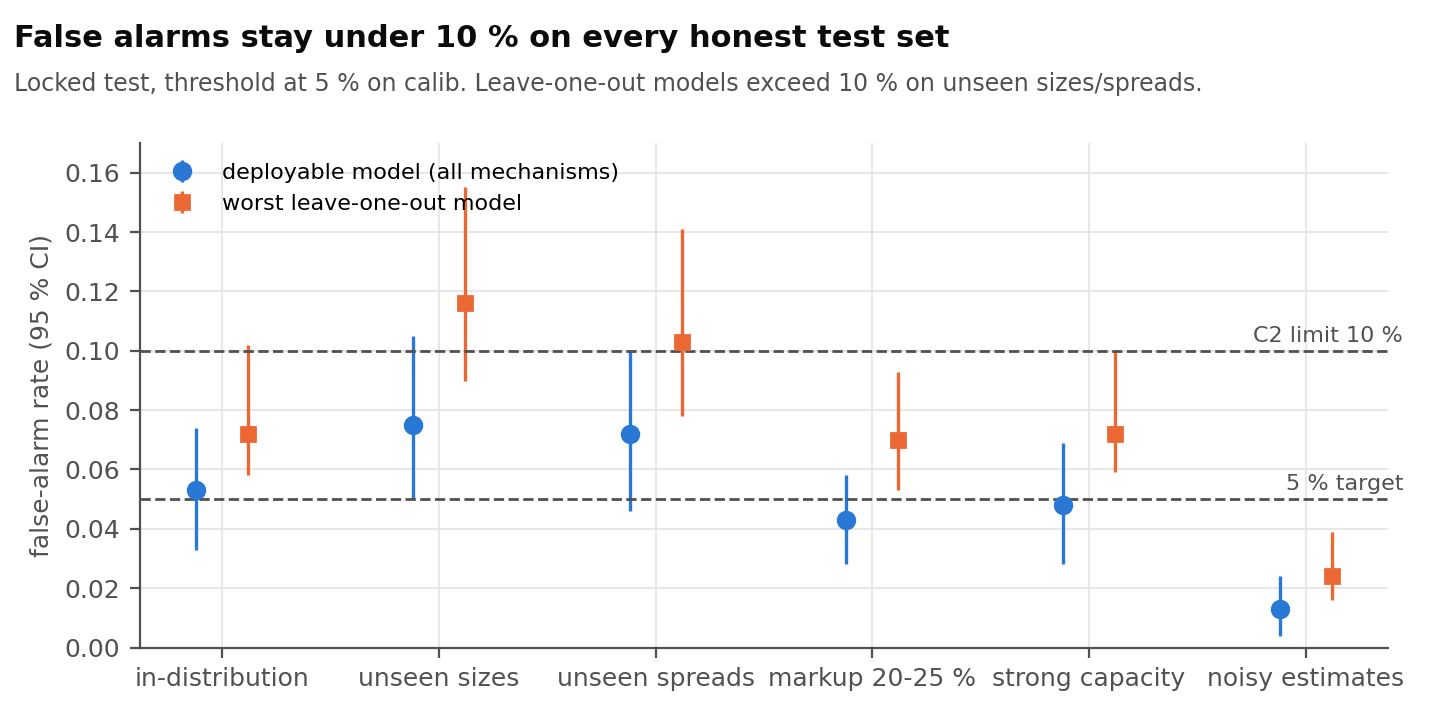
\includegraphics[width=\linewidth]{../figures/fig3_locked_false_alarms.png}
\caption{Share of honest test markets flagged, deployable model and worst leave-one-scheme-out model (95\,\% CIs).}
\end{figure}

The deployable detector flags at most 7.5\,\% of honest markets on any honest test set, inside the 10\,\% limit, including market sizes and cost spreads it never trained on. The threshold was set once, at 5\,\% false alarms on separate honest calibration markets, and then applied unchanged to six honest test sets. Three are the in-distribution and shifted conditions; three are stress tests that look suspicious to a naive screen: high honest markups (20--25\,\%), strong capacity effects that make honest wins rotate, and noisy estimates and costs. None of them pushes the deployable model past 10\,\%. High markups do not raise false alarms, which confirms that the features ignore the price level.

The deployable model is trained on all eight schemes. The grey dots show the worst of the eight leave-one-scheme-out models, which are trained on seven. Those exceed 10\,\% on unseen sizes (11.6\,\%) and unseen spreads (10.3\,\%), so the false-alarm guarantee holds for the full model, not for every partial one.

% ---------------------------------------------------------------- WHAT DROVE
\section{What drove the result}

The gain comes from the dependence features; the change scans and the Bayesian sequential layer add nothing measurable. These numbers are from the validation split (10 seeds), where designs were chosen. The locked test was not used for any choice.

\begin{table}[H]
\centering
\small
\begin{tabular}{@{}lr@{}}
\toprule
Design (validation) & Macro AUC [95\,\% CI] \\
\midrule
All feature groups & 0.862 [0.853, 0.871] \\
Without change scans & 0.864 [0.856, 0.873] \\
Without the sequential layer & 0.862 [0.853, 0.871] \\
Without dependence features & 0.801 [0.790, 0.811] \\
Dependence features only & 0.826 [0.814, 0.836] \\
Literature screens only & 0.806 [0.795, 0.816] \\
Sequential layer only & 0.549 [0.530, 0.566] \\
Change scans only & 0.494 [0.480, 0.506] \\
\bottomrule
\end{tabular}
\caption{Feature-group ablations on the validation split.}
\end{table}

\begin{figure}[H]
\centering
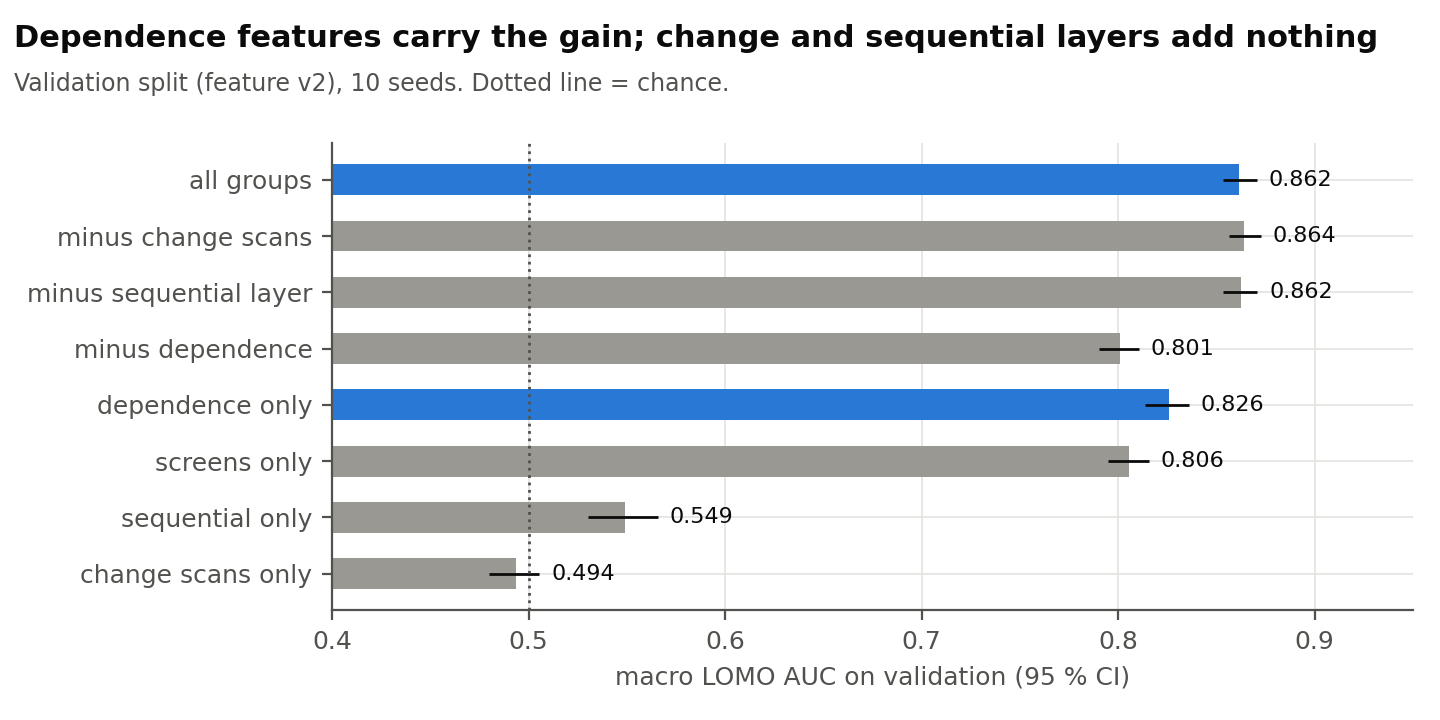
\includegraphics[width=0.9\linewidth]{../figures/fig6_ablation.png}
\caption{Validation ablation of feature groups (feature version 2).}
\end{figure}

\textbf{Improvement attempts.} Each was tried on validation with a stated hypothesis and a test that could falsify it, and was kept only if validation improved. A pre-set rule stopped a line of work after three attempts without a gain.

\begin{table}[H]
\centering
\small
\begin{tabular}{@{}p{1.8cm}p{7.2cm}p{5.4cm}@{}}
\toprule
Attempt & Idea & Outcome \\
\midrule
I1 & Add a second shuffle (each firm's bids reordered across tenders) & Kept: macro AUC 0.847 $\to$ 0.862 \\
I2 & Participation features plus a knowledge-directed tail score fused with the model & No gain (0.864); helped bid suppression, hurt noisy and intermittent cartels \\
I3 & Use the single most suspicious firm pair instead of the top three & Dropped at prototype: no gain on small cartels \\
I4 & Constrain the model to move in the expected collusion directions & No gain (0.867, within the confidence interval) \\
W2-1 to W2-3 & Three ways to detect a cartel that starts and stops (pair-closeness scan, segment excess, window scan) & No gain; the last was reverted \\
\bottomrule
\end{tabular}
\caption{Improvement attempts on the validation split.}
\end{table}

Only I1 survived, so the frozen design is the model with I1 and nothing else. Both lines of work, the detector features and the change detection, ended under the stop rule.

% ---------------------------------------------------------------- REAL DATA
\section{Real-data test}

On real cartel cases the detector beat the literature screens in Italy (+0.144 AUC) but not in Japan or Brazil. An alarm threshold set on two countries did not carry over to the third.

\subsection{The data}

The data are real per-bid records from prosecuted bid-rigging cases, published with García Rodríguez et al.\ (2022), \emph{Collusion detection in public procurement auctions with machine learning algorithms}, \emph{Automation in Construction} 133, 104047 (\url{https://www.sciencedirect.com/science/article/pii/S0926580521004982}). The supplementary file's checksum is recorded in the experiment log. Each bid comes with the bidding firm's ID, the buyer's pre-tender estimate, and whether the bidder was a cartel member. Three of the six country sets have everything the detector needs:

\begin{table}[H]
\centering
\small
\begin{tabular}{@{}llrrp{5.2cm}@{}}
\toprule
Country & Case & Tenders & Collusive & Auction format \\
\midrule
Italy & Turin road construction & 278 & 143 & Average-bid (the winner is not the lowest bid) \\
Japan & Okinawa construction & 1{,}080 & 123 & Lowest bid wins, with a price floor \\
Brazil & Petrobras infrastructure & 101 & 33 & Lowest bid wins \\
\bottomrule
\end{tabular}
\caption{The three real-data cases.}
\end{table}

The two Swiss sets have no firm IDs and the US set has no estimate, so they were left out.

\subsection{Why tenders, not markets}

The simulator scores whole markets of repeated tenders. Real tenders do not come grouped that way. Windows of consecutive tenders were checked first: in Japan no window of 20--40 tenders was mostly collusive, and no firm bid six or more times inside any window. Grouping tenders by shared bidders produced repeated markets only in Italy. So each tender was scored on its own.

\subsection{How it was tested}

The design was written down and approved before the run, and the run was done once; the script refuses to repeat it.

\begin{enumerate}[leftmargin=2em]
\item For each tender, compute the literature screens of its own bids.
\item For every pair of its bidders, measure how that pair behaved in all other tenders of the same country: whether their bids co-move, how often they bid within 3\,\% of each other, and how often they bid on the same tenders. Excluding the tender itself keeps the feature honest; a test checks this against a brute-force recomputation.
\item Convert every feature to a within-country percentile, so currencies and project sizes compare across countries. This uses each country's unlabelled data and is disclosed as a design choice.
\item Train on two countries and test on the third, three times over. Labels come from the source paper's tender labels.
\item Set the alarm threshold at 5\,\% false alarms on the training countries' competitive tenders, then measure false alarms on the held-out country.
\item Compute confidence intervals with a block bootstrap over tenders in time order (blocks of 20, 1{,}000 resamples), paired across methods.
\end{enumerate}

\subsection{Results}

\begin{table}[H]
\centering
\small
\begin{tabular}{@{}lllllll@{}}
\toprule
Held-out & Detector AUC & Screens-only AUC & Difference & Best single screen & False alarms & Precision@10\,\% (base) \\
\midrule
Italy & 0.779 [0.668, 0.876] & 0.635 & \textbf{+0.144} [0.078, 0.234] & spread 0.676 & 0.7\,\% & 0.93 (0.51) \\
Japan & 0.691 [0.627, 0.758] & 0.674 & +0.018 [$-$0.032, 0.069] & CV 0.739 & 26.5\,\% & 0.26 (0.11) \\
Brazil & 0.742 [0.661, 0.850] & 0.755 & $-$0.013 [$-$0.109, 0.177] & CV 0.873 & 8.8\,\% & 0.50 (0.33) \\
\bottomrule
\end{tabular}
\caption{Real-data results, leave-one-country-out, tender level (95\,\% CIs).}
\end{table}

\begin{figure}[H]
\centering
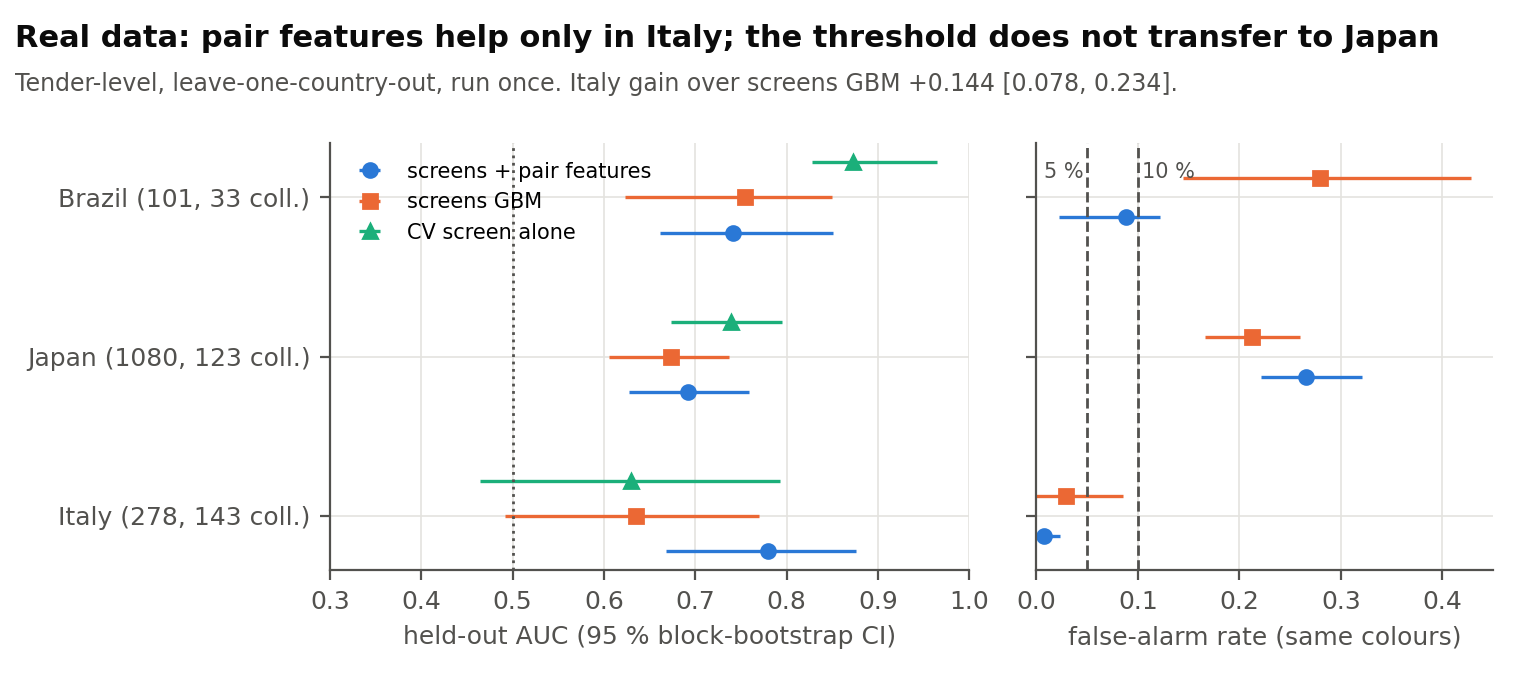
\includegraphics[width=\linewidth]{../figures/fig7_real_data_lodo.png}
\caption{Real-data AUC and false-alarm rates by held-out country (block-bootstrap 95\,\% CIs).}
\end{figure}

\textbf{What it shows.}
\begin{itemize}
\item \emph{Italy:} the pair features clearly help, beat every single screen, and false alarms are near zero. Italy is the only country where the same firms meet repeatedly, which is the setting the method is built for.
\item \emph{Japan:} no gain over the screens, a plain CV screen is at least as good, and false alarms reach 26.5\,\% instead of 5\,\%.
\item \emph{Brazil:} no gain over the screens, and significantly worse than the CV screen alone ($-$0.131 [$-$0.247, $-$0.013]). Most firms bid only once, so pair features have almost no history to use.
\end{itemize}

Each country is one cartel case, so these are three case studies, not a general detection rate.

% ---------------------------------------------------------------- LIMITATIONS
\section{Limitations}

The detector misses quiet cartels, cannot see uniform price-level collusion, and does not carry over to other bid-generating processes without recalibration.

\begin{itemize}
\item \textbf{Four schemes stay below AUC 0.85} (worst condition in brackets): partial cartel with a fringe 0.672 (0.621), bid suppression 0.744 (0.677), noisy or defecting cartel 0.823 (0.775), intermittent cartel 0.871 (0.849 at unseen spreads). A cartel of 2--3 firms leaves a trace in one or two of up to 435 firm pairs over only 20--60 tenders; this may be close to an information limit (a hypothesis, not proven). Bid suppression's own signal, missing bids, cannot be learned when that scheme is held out.
\item \textbf{Uniform-markup collusion is invisible from bids alone} (AUC 0.478). Without cost data, a common price rise looks like higher costs. This is an identification limit, shown on purpose as a control.
\item \textbf{Transfer to the old reinforcement-learning simulator fails.} The frozen detector was applied to scripted episodes of the earlier environment (20 rounds by 20 firms). With the benchmark's threshold it flagged 99.7\,\% of honest episodes, and against those honest episodes most cartel AUCs fell below 0.5 (cover cartels 0.31--0.74, target-pricing cartels 0.006--0.43). With the threshold refitted on that environment's own honest episodes, false alarms dropped to 7.0\,\% but cartels were flagged at 0--15\,\%, no better than honest markets. AUCs do not change with the threshold, so the failure is in how the model ranks markets, not in calibration. A likely cause (untested): honest bidders there all anchor to the last winning price, so their bids co-move, which the detector reads as coordination.
\item \textbf{Thresholds need per-market calibration.} Both the real data (26.5\,\% false alarms in Japan) and the old simulator show that a threshold set elsewhere does not carry over.
\item \textbf{Real-data evidence is three cases}, one cartel per country, scored tender by tender with the source paper's thresholded labels. Italy's average-bid auction changes what the gap and relative-distance screens mean.
\item \textbf{The detector scores markets or tenders, not firms.} It does not name cartel members.
\item \textbf{Cartels are imposed, not equilibrium behaviour.} The schemes and their parameter ranges are design choices, and honest firms follow rules rather than strategy.
\end{itemize}

% ---------------------------------------------------------------- FUTURE WORK
\section{Future work}

The most valuable next steps are better honest-behaviour modelling and calibration, more real cartel cases, and a strategic version in which the cartel chooses how to evade the detector. Any new design goes through the same protocol: validation first, then one locked run.

\subsection{To finish the current paper}
\begin{itemize}[label=$\square$]
\item Write the related-work section, with every citation checked against its source.
\item Choose the venue (workshop or benchmark track) and fit the 4--6 page format.
\item Decide whether the old-simulator result goes in the main text or the appendix.
\end{itemize}

\subsection{To improve detection of the weak schemes}

\begin{table}[H]
\centering
\small
\begin{tabular}{@{}p{6.2cm}p{6cm}p{2.8cm}@{}}
\toprule
Work item & Why & Targets \\
\midrule
Firm-level scoring: find the most suspicious group of firms, not just a market score & A 2--3 firm cartel is diluted in a market-level score; naming the group also makes results usable by an authority & Partial cartel, noisy cartel \\
Participation models that predict who should bid, then flag who is missing & Suppression's signal is absent bids; it needs an explicit model of expected participation & Bid suppression \\
Longer histories and window-aware features trained on intermittent patterns & Short markets (20--60 tenders) limit what a start-stop cartel reveals & Intermittent cartel \\
A measured information limit: how many tenders a $k$-firm cartel needs before any detector can see it & Tells whether the misses are fixable or a hard limit & All weak schemes \\
\bottomrule
\end{tabular}
\caption{Planned work to improve detection of the weak schemes.}
\end{table}

\subsection{To make it robust across settings}
\begin{itemize}
\item Richer honest-bidding models, including firms that anchor to the last winning price as in the old simulator, added to training so the detector stops reading honest co-movement as collusion.
\item Per-market calibration: set the alarm threshold from each market's own honest history, or from a small labelled sample, instead of carrying one threshold over.
\item Domain checks before deployment: a test that flags when a new market's honest bids look unlike the training data.
\end{itemize}

\subsection{More real data}
\begin{itemize}
\item Find further per-bid datasets with cartel labels and firm IDs (for example other national procurement cases), so that leave-one-cartel-out tests have more than three cases. Any download needs approval first.
\item Score at market level wherever firms meet repeatedly, as in Italy, where the method worked.
\end{itemize}

\subsection{A strategic follow-up (second paper)}
\begin{itemize}
\item Turn detection into a leader--follower game: the regulator commits to the frozen detector, and the cartel chooses its scheme parameters (inflation, cover gap, defection rate, active share) to maximise profit while staying under the alarm. The result is an evasion frontier: how much profit a cartel must give up to stay hidden.
\item This links back to the original project's Bayesian sequential regulator. It would need a payoff model in which collusion actually pays, which was the lesson of the reinforcement-learning work, so step one is a payoff check across schemes before any game is run.
\end{itemize}

% ---------------------------------------------------------------- FILES
\section{Files and sources}

All numbers in this report come from logged result files in the project repository (\texttt{Jayati ma'am project-v2}, branch \texttt{benchmark-v1}).

\begin{table}[H]
\centering
\small
\begin{tabular}{@{}p{5.6cm}p{8.4cm}@{}}
\toprule
What & File \\
\midrule
Locked test & \texttt{results/locked\_1\_full\_gbm.md}, \texttt{results/locked\_runs.jsonl} \\
Validation runs & \texttt{results/validation\_v1} to \texttt{validation\_v4} (\texttt{.md}, \texttt{.json}) \\
Real-data run & \texttt{results/real\_lodo\_1.md}; design in \texttt{docs/real\_data\_design.md} \\
Old-simulator transfer & earlier repo, branch \texttt{new-detector-check}: \texttt{results/new\_detector\_on\_old\_env/}, \texttt{results/new\_detector\_recalibrated/} \\
Every run with its hypothesis and outcome & \texttt{docs/experiment\_log.md} \\
Claims and their evidence & \texttt{docs/claims\_table.md} \\
Figures and their data tables & \texttt{docs/figures/} \\
Paper outline & \texttt{docs/paper\_outline.md} \\
\bottomrule
\end{tabular}
\caption{Where each result is stored.}
\end{table}

\textbf{Real data.} García Rodríguez, Rodríguez-Montequín, Ballesteros-Pérez, Love and Signor (2022), \emph{Collusion detection in public procurement auctions with machine learning algorithms}, \emph{Automation in Construction} 133, 104047, supplementary data.

\end{document}
